\documentclass[acmlarge,screen]{acmart}

\usepackage[utf8]{inputenc}
\usepackage[brazil]{babel}
\usepackage{indentfirst}
\usepackage{graphicx}
\usepackage{listings} 
\usepackage{graphics}

\lstset{language=Gnuplot}

\copyrightyear{2019}
\acmYear{2019}
\setcopyright{acmlicensed}
\acmConference[Woodstock '18]{Woodstock '18: ACM Symposium on Neural Gaze Detection}{June 03--05, 2018}{Woodstock, NY}
\acmPrice{15.00}
\acmDOI{10.1145/1122445.1122456}
\acmISBN{978-1-4503-9999-9/18/06}

\setcopyright{acmcopyright}
\acmJournal{CSUR}
\acmYear{2019}\acmVolume{1}\acmNumber{1}\acmArticle{1}\acmMonth{3}
\acmDOI{10.1145/1122445.1122456}

\begin{document}

\title{Lista 1 - Respostas}

\settopmatter{printacmref=false}

\author{Samuel Lucas de Moura Ferino}
\authornote{Bacharelando do curso de Tecnologia da Informação (BTI) na Universidade Federal do Rio Grande do Norte (UFRN). }
\email{samuellucas97@ufrn.edu.br}
\affiliation{%
  \institution{2016.039.761}
}

\begin{abstract}
Neste documento encontram-se as respostas relativas a primeira lista de exercícios da disciplina DIM0404 CÁLCULO NUMÉRICO PARA  CIÊNCIA DA COMPUTAÇÃO. Diante disso, no tópico Questão 1 há inicialmente uma breve explicação do enunciado sendo seguida pela resolução adotada. Além disso, de igual modo, nas demais seções: Questão 2 e Questão 3, também há uma breve explicação do enunciado seguida pela solução usada.    
\end{abstract}


\maketitle

\section{Introdução}
Trata-se do relatório das soluções utilizadas para resolver a 1ª lista de exercícios referente aos 2,0 pontos da 1ª unidade da disciplina DIM0404 CÁLCULO NUMÉRICO PARA  CIÊNCIA DA COMPUTAÇÃO lecionada pelo Dr. Rafael Beserra Gomes. Portanto, nas seções Questão 1, Questão 2 e Questão 3 encontram-se os enunciados e as resoluções adotadas.

\section{Questão 1}

O enunciado segue assim:
\newline
\begin{enumerate}
    \item Considere a função $f(x) = x^3 - 2x^2 - x + 2$. Plote em um mesmo gráfico:
    
    \begin{enumerate}
        \item $f(x)$ com a legenda \textcolor{red}{``função cúbica``} no intervalo de x [−1.5, 2.5]
        \item a reta tangente no ponto ( 1, $f(1)$ ) com a legenda \textcolor{red}{reta tangente em x = 1 }
        \item 4 pontos: ( 1, $f(1)$ ), a interseção entre a reta tangente e o eixo x, os dois pontos críticos (e as respectivas retas tangentes) 

    
    \end{enumerate}
    
    Adicione um grid, eixo x e eixo y.
    
\end{enumerate}



Diante disso, o script do gnuplot que cria o gráfico é o seguinte:

\begin{lstlisting}[htb]
set terminal png size 900, 600 enhanced
set output 'exercicio1.png'
set encoding utf8
set grid
set xlabel "Coordenada X"
set ylabel "Coordenada Y"
set key below
set xzeroaxis
set yzeroaxis
plot [-1.5:2.5] x**3 - 2*(x**2) -x + 2 title 'função cúbica' linestyle 7 with linespoint,\
-2*x + 2 title 'reta tangente em x = 1' lw 3 lc "grey",\
(14*sqrt(7) - 34)/27 + 2 title 'reta tangente em x = (2 - sqrt(7))/3' lw 2 lc "green",\
(-14*sqrt(7) - 34)/27 + 2 title 'reta tangente em x = (2 + sqrt(7))/3' lw 2 lc "magenta",\
'dados_1_0.pts' title '( 1, 0 )' lw 8,\
'dados_pontoCritico_1.pts' title '( (2 - sqrt(7))/3, 14*sqrt(7) - 34)/27 + 2 )' lw 8,\
'dados_pontoCritico_2.pts' title '( (2 + sqrt(7))/3, -14*sqrt(7) - 34)/27 + 2 )' lw 8,\
\end{lstlisting}
 
 Além disso, a imagem produzida pelo script apresentado é a seguinte:
 
\begin{figure}[htb]
    \centering
    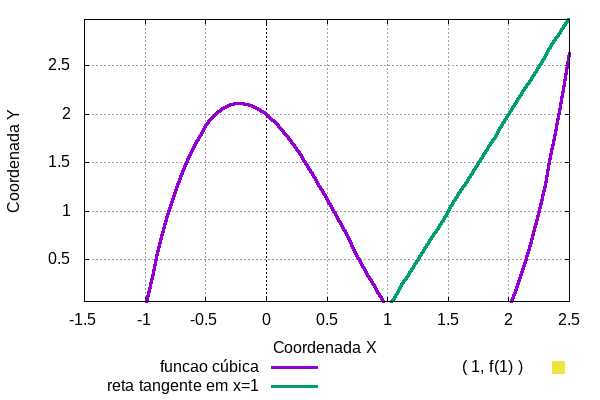
\includegraphics[scale=0.5]{exercicio1.png}
    \caption{Gráfico correspondente a questão 1}
    \label{fig:my_label}
\end{figure}

\section{Questão 2}

O enunciado segue assim:
\newline
\begin{enumerate}
    \item Estime os pontos da função $f(x)$ no intervalo [-6:6] dado que (e somente a partir dessas informações):
    
    \begin{enumerate}
        \item $f(0) = 1$
        \item $f'(x) = cos(x) - x*sen(x)$
        
    \end{enumerate}
    
    Grave os pontos estimados em um arquivo e o plote-os com \newline
    \textbf{plot \textcolor{red}{``arquivos.pts``} with lp, x*cos(x) + 1}
    
\end{enumerate}


Diante disso, o código do programa que descobre esse pontos e salva-os em um arquivo é o seguinte



Em seguida, o script do gnuplot que cria o gráfico é o seguinte:

\begin{lstlisting}[htb]
set terminal png size 900, 600 enhanced
set output 'exercicio2.png'
set grid
set xzeroaxis
set yzeroaxis
set xlabel "Coordenada X"
set ylabel "Coordenada Y"
set key below
plot [-6:6] 'arquivos.pts' title 'aproximação de x*cos(x) + 1'with lp lc 2 lw 2,\
 x*cos(x)+1 lc 5 lw 3 
\end{lstlisting}
 
 Além disso, a imagem produzida pelo script apresentado acima é a seguinte:
 
\begin{figure}[htb]
    \centering
    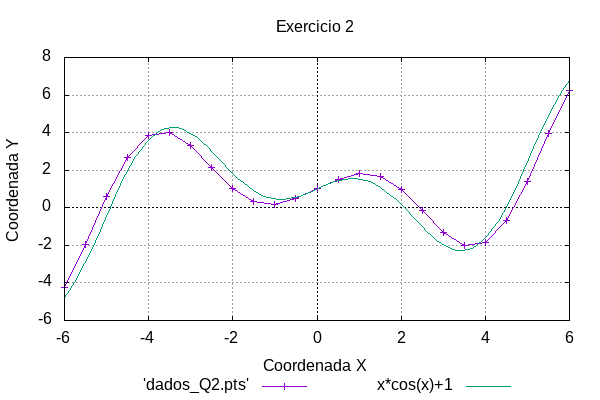
\includegraphics[scale=0.5]{exercicio2.png}
    \caption{Gráfico correspondente a questão 2}
    \label{fig:my_label}
\end{figure}


\section{Questão 3}

O enunciado segue assim:
\newline
Plot em um mesmo gráfico a função $f(x) = xcos(x)$ e sua aproximação pela série de taylor.
\section{CONSIDERAÇÕES FINAIS}



\end{document}
